\documentclass[a4paper, 12pt]{article}

%\usepackage{cmap}
\usepackage[T2A]{fontenc}
\usepackage[utf8]{inputenc}
\usepackage[english, russian]{babel}
\usepackage{graphicx}
\usepackage[top=1in, bottom=1in, left=3.2cm, right=2.6cm]{geometry}
\graphicspath{./}
\usepackage{biblatex}
\addbibresource{lib.bib}
\linespread{1.5}
\usepackage{ragged2e}
\justifying
\usepackage{listings}
\usepackage{color}
\usepackage{amsmath}


\begin{document}
	
\begin{titlepage}
	\fontsize{12pt}{12pt}\selectfont
	\begin{figure}[t!]
		\centering
		
\includegraphics[scale=0.8]{bmstu}
	\end{figure}
	
	\noindent\rule{15cm}{3pt}
	\newline\newline
	\noindent 
	ФАКУЛЬТЕТ 
	\underline{«Информатика и системы управления»} \newline
	
	\noindent КАФЕДРА \underline{«Программное обеспечение ЭВМ и информационные технологии»}\newline\newline\newline\newline\newline
	
	\centering {\Large \textbf{Отчет по лабораторной работе № 1}}
	\vspace{4mm}
	
	\centering {\Large \textbf{По курсу:} Моделирование
		\vspace{8mm}}
	\\ \centering {\Large \textbf{На тему:} Изучение функции распределения и функции плотности распределения случайной величины}
	\vspace{20mm}
	
	
	\begin{flushright}
		{\small	\textbf{Студент:}\\ Турсунов Жасурбек Рустамович \\ \textbf{Группа:} ИУ7-76Б
			\vspace{3mm}
			\\\textbf{Преподователь:} \\ Рудаков Игорь Владимирович }
	\end{flushright}
	
	\begin{center}
		\vfill
		Москва, \the\year
		~г.
	\end{center}
\end{titlepage}

\tableofcontents
\clearpage
\newpage


\section{{Задание}}

\hspace*{5mm} Реализовать программу для построения графиков функции и плотности для следующих распределений:
\begin{itemize}
	\item равномерное распределение;
	\item нормальное распределение (вариант 15).
\end{itemize}

\section{{Теоритическая часть}}
\subsection{Равномерное распределение}

Непрерывное равномерное распределение - распределение случайной вещественной величины, принимающей значения, принадлежащие некоторому промежутку конечной длины, характеризующееся тем, что плотность вероятности на этом промежутке почти всюду постоянна.

Плотность распределения представлена в формуле \ref{eq:uniform_density}.

\begin{equation}\label{eq:uniform_density}
	f_X (x) =
	\begin{cases}
		\frac{1}{b-a}, x \in [a,b] \\
		0, x \notin [a, b] \\
	\end{cases}
\end{equation}

Функция распределения представлена в формуле \ref{eq:uniform_function}.

\begin{equation}\label{eq:uniform_function}
	F_X (x) =
	\begin{cases}
		0, x < a \\
		\frac{x - a}{b - a}, a \le x < b \\
		1, x \geq b \\
	\end{cases}
\end{equation}

\subsection{Нормальное распределение}

Нормальное распределение~--- распределение вероятностей, которое в одномерном случае задаётся функцией плотности вероятности, совпадающей с функцией Гаусса.

Плотность распределения представлена в формуле \ref{eq:gauss_density}.

\begin{equation}\label{eq:gauss_density}
	f_X (x) = \frac{1}{\sigma \sqrt{2 \pi}} e^{-\frac{(x - \mu)^2}{2 \sigma^2}}
\end{equation}

Функция распределения представлена в формуле \ref{eq:gauss_function}.

\begin{equation}\label{eq:gauss_function}
	F (x) = \frac{1}{\sigma \sqrt{2\pi}} \int_{-\infty}^x e^{-\frac{(t- \mu)^2}{2 \sigma^2}} dt
\end{equation}

\section{{Результаты}}
\subsection{Равномерное распределение}
\begin{figure}[h!]
	\centering 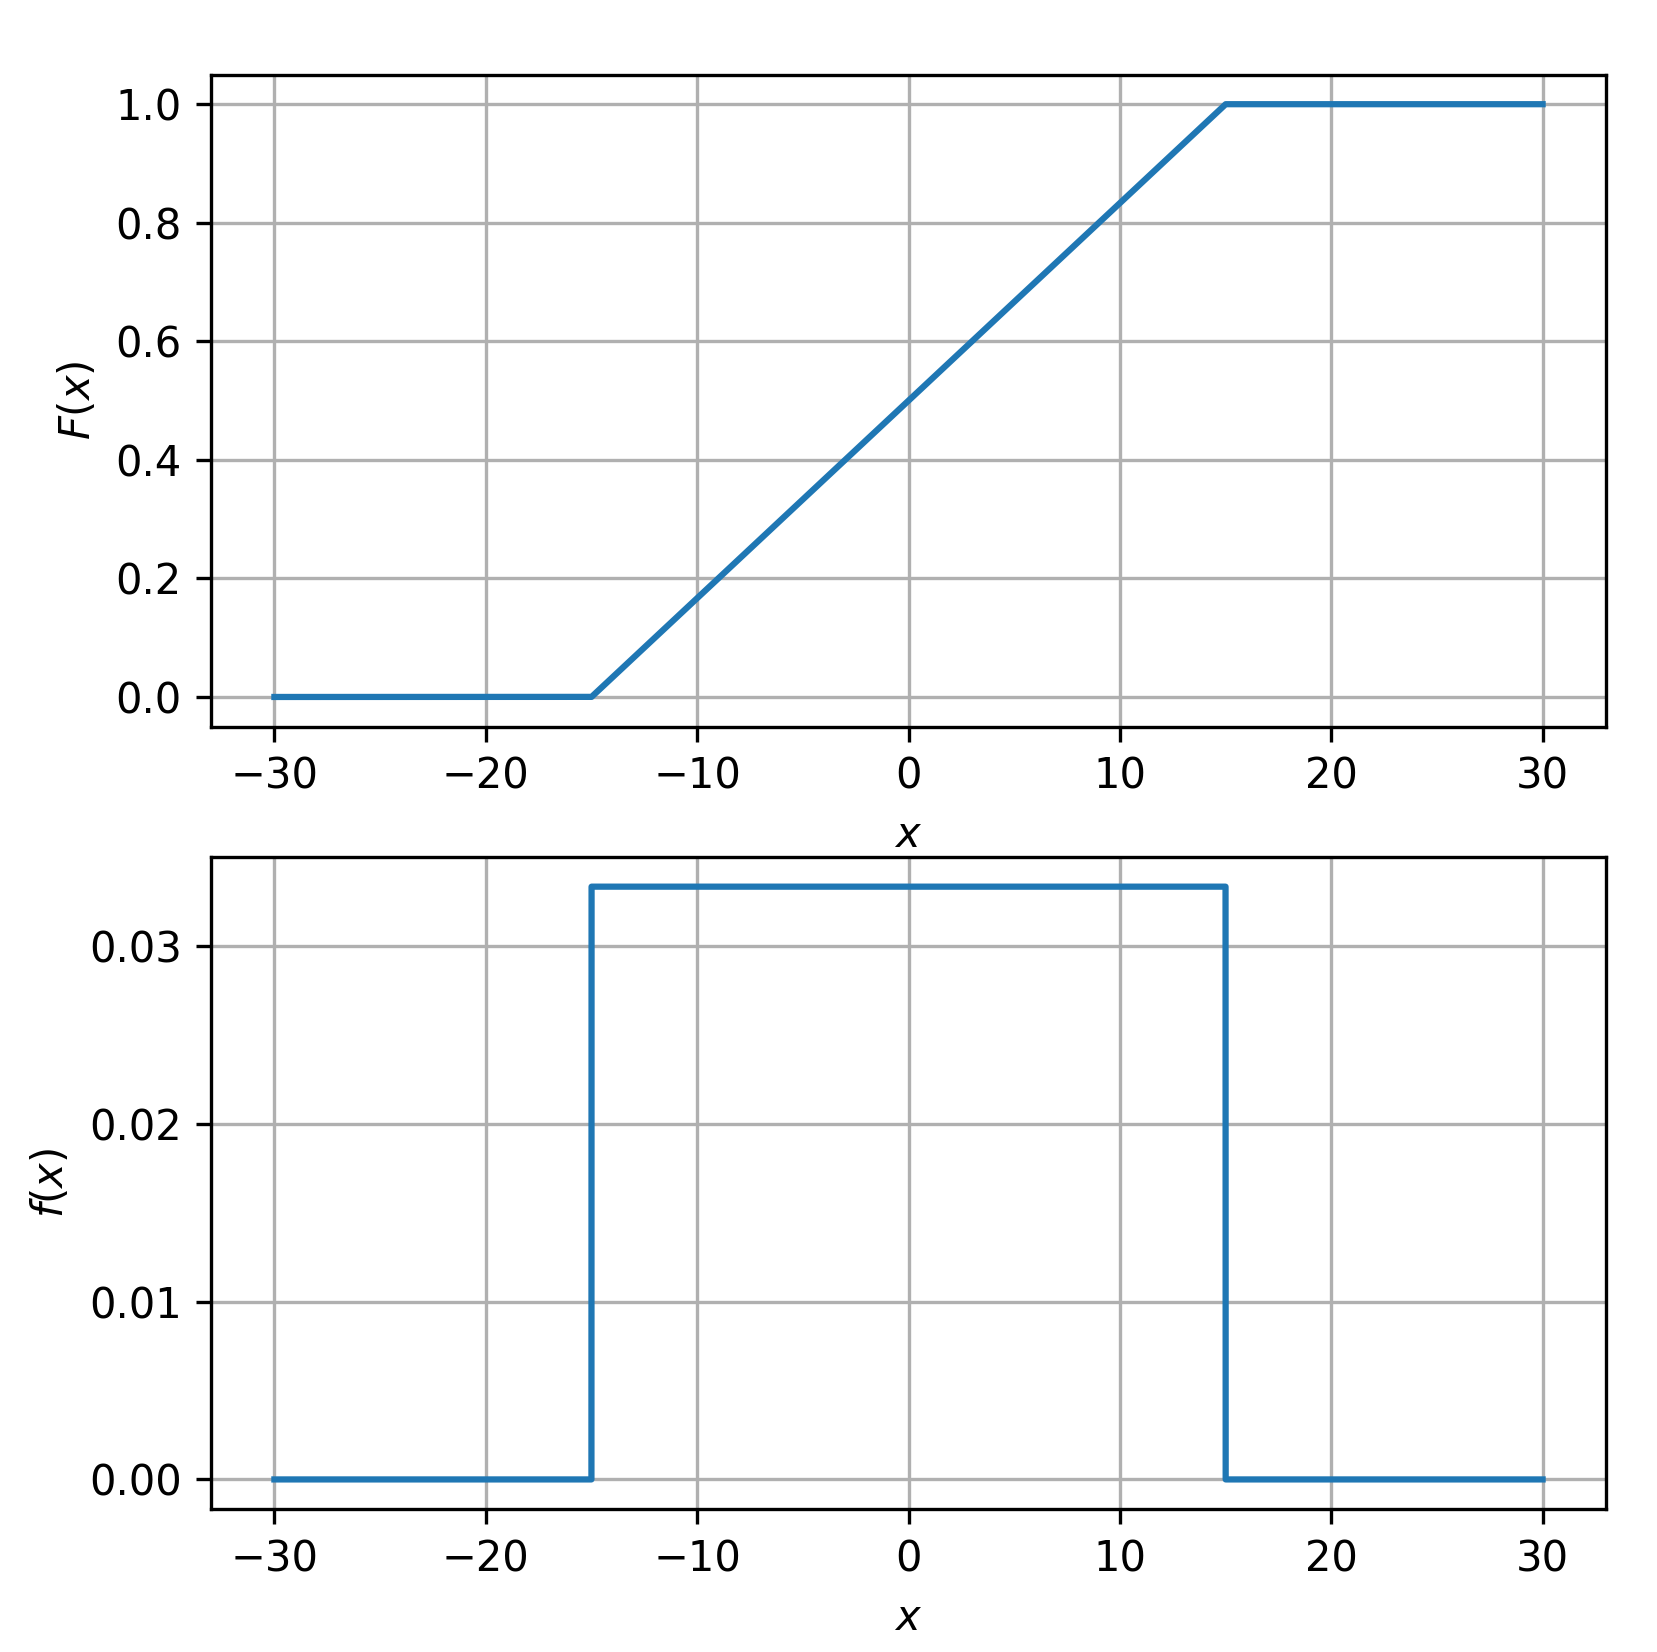
\includegraphics[scale=0.8]{ud1}
	\centering\caption{Равномерное распределение при a = -15, b = 15}
\end{figure}
\clearpage
\newpage
\begin{figure}[t!]
	\centering 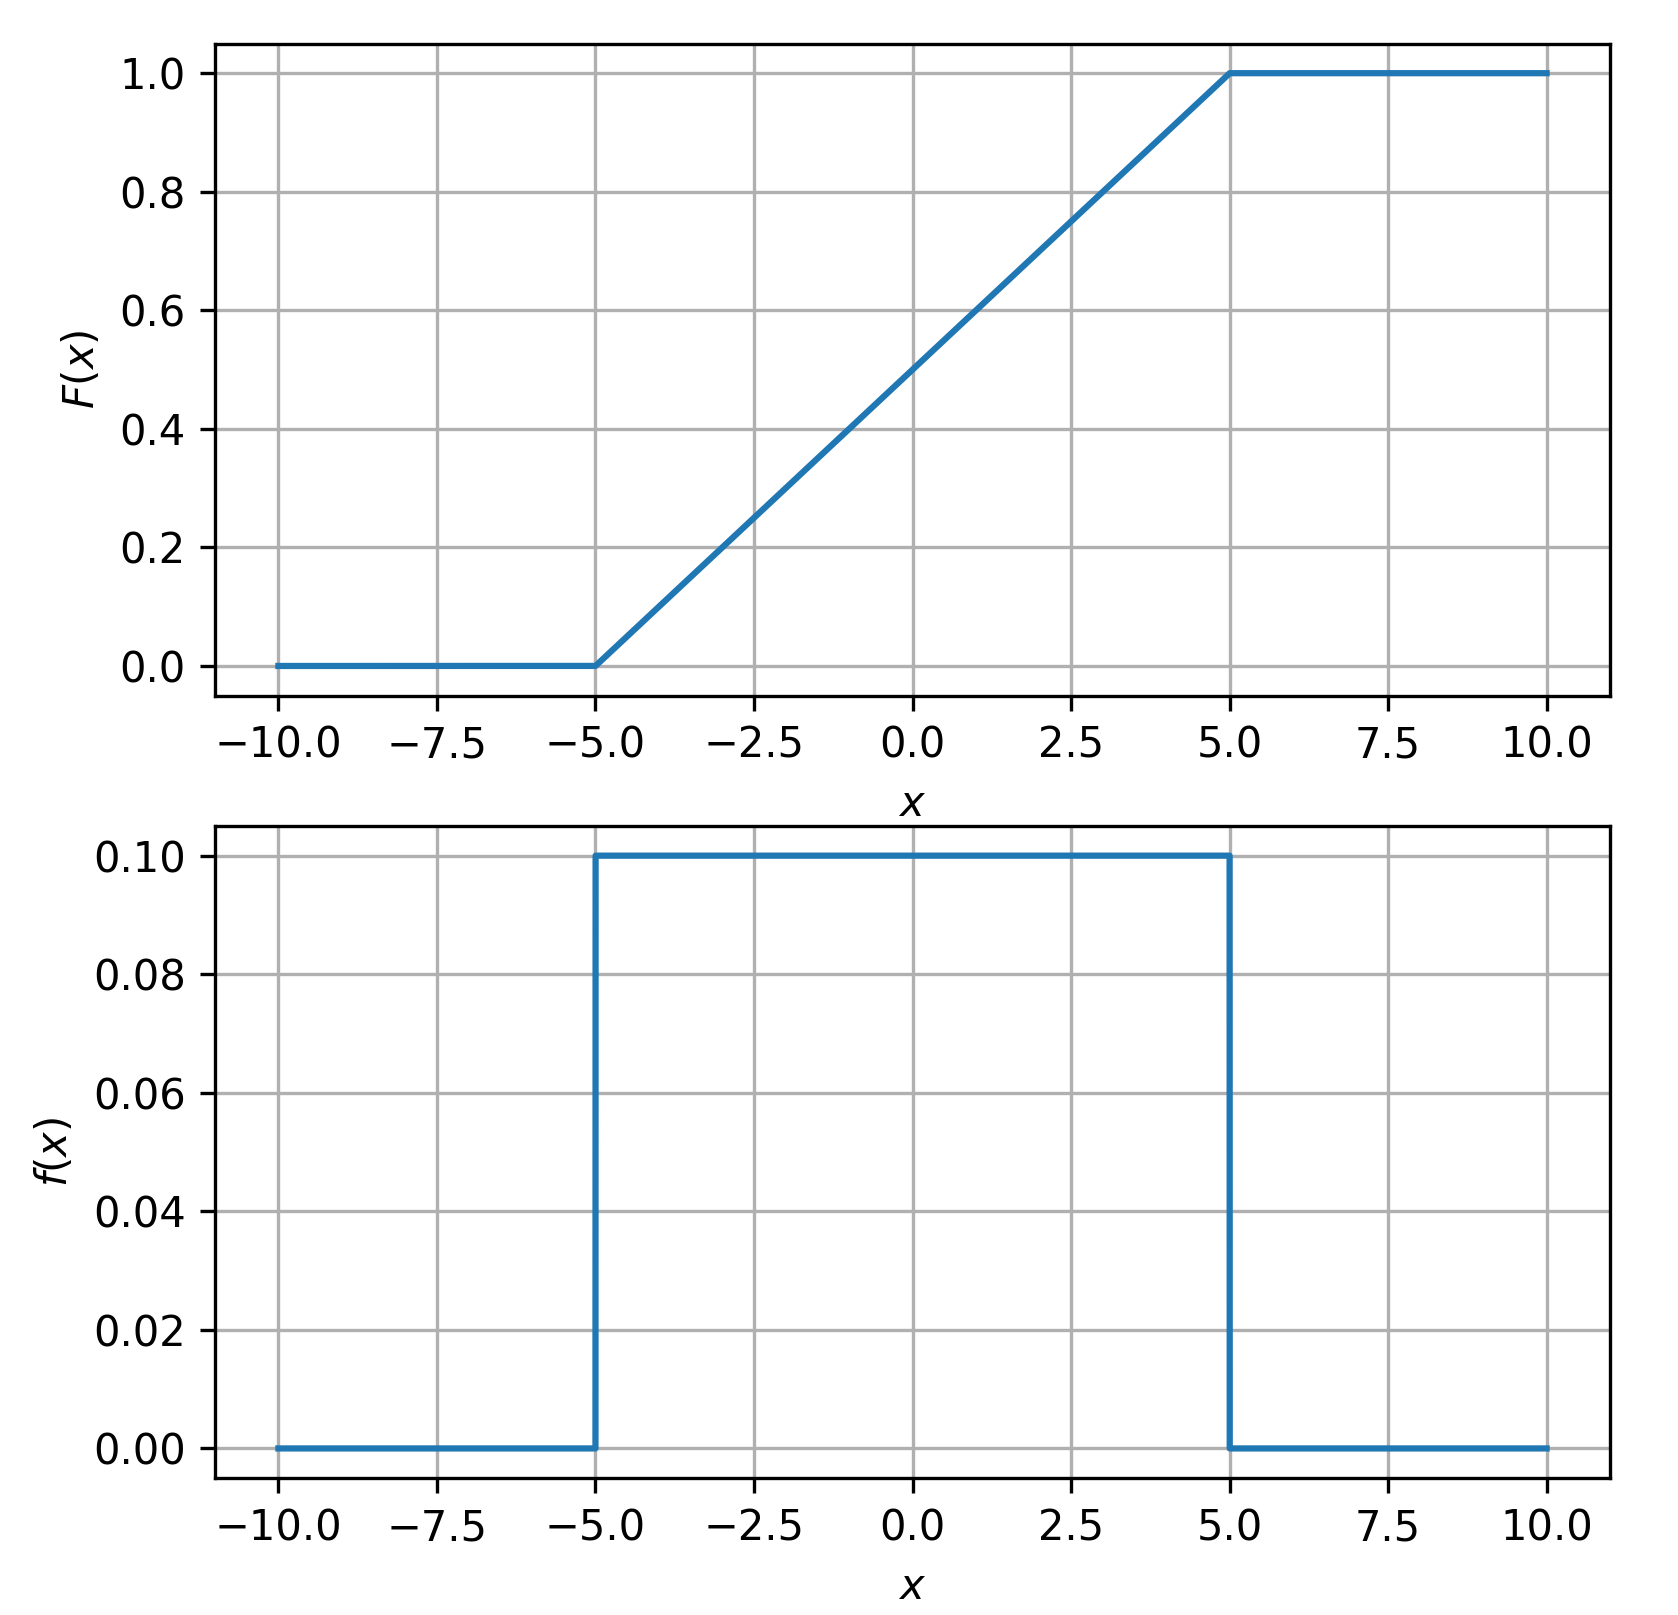
\includegraphics[scale=0.8]{ud2}
	\centering\caption{Равномерное распределение при a = -5, b = 5}
\end{figure}
\clearpage
\newpage
\subsection{Нормальное распределение}
\begin{figure}[h!]
	\centering 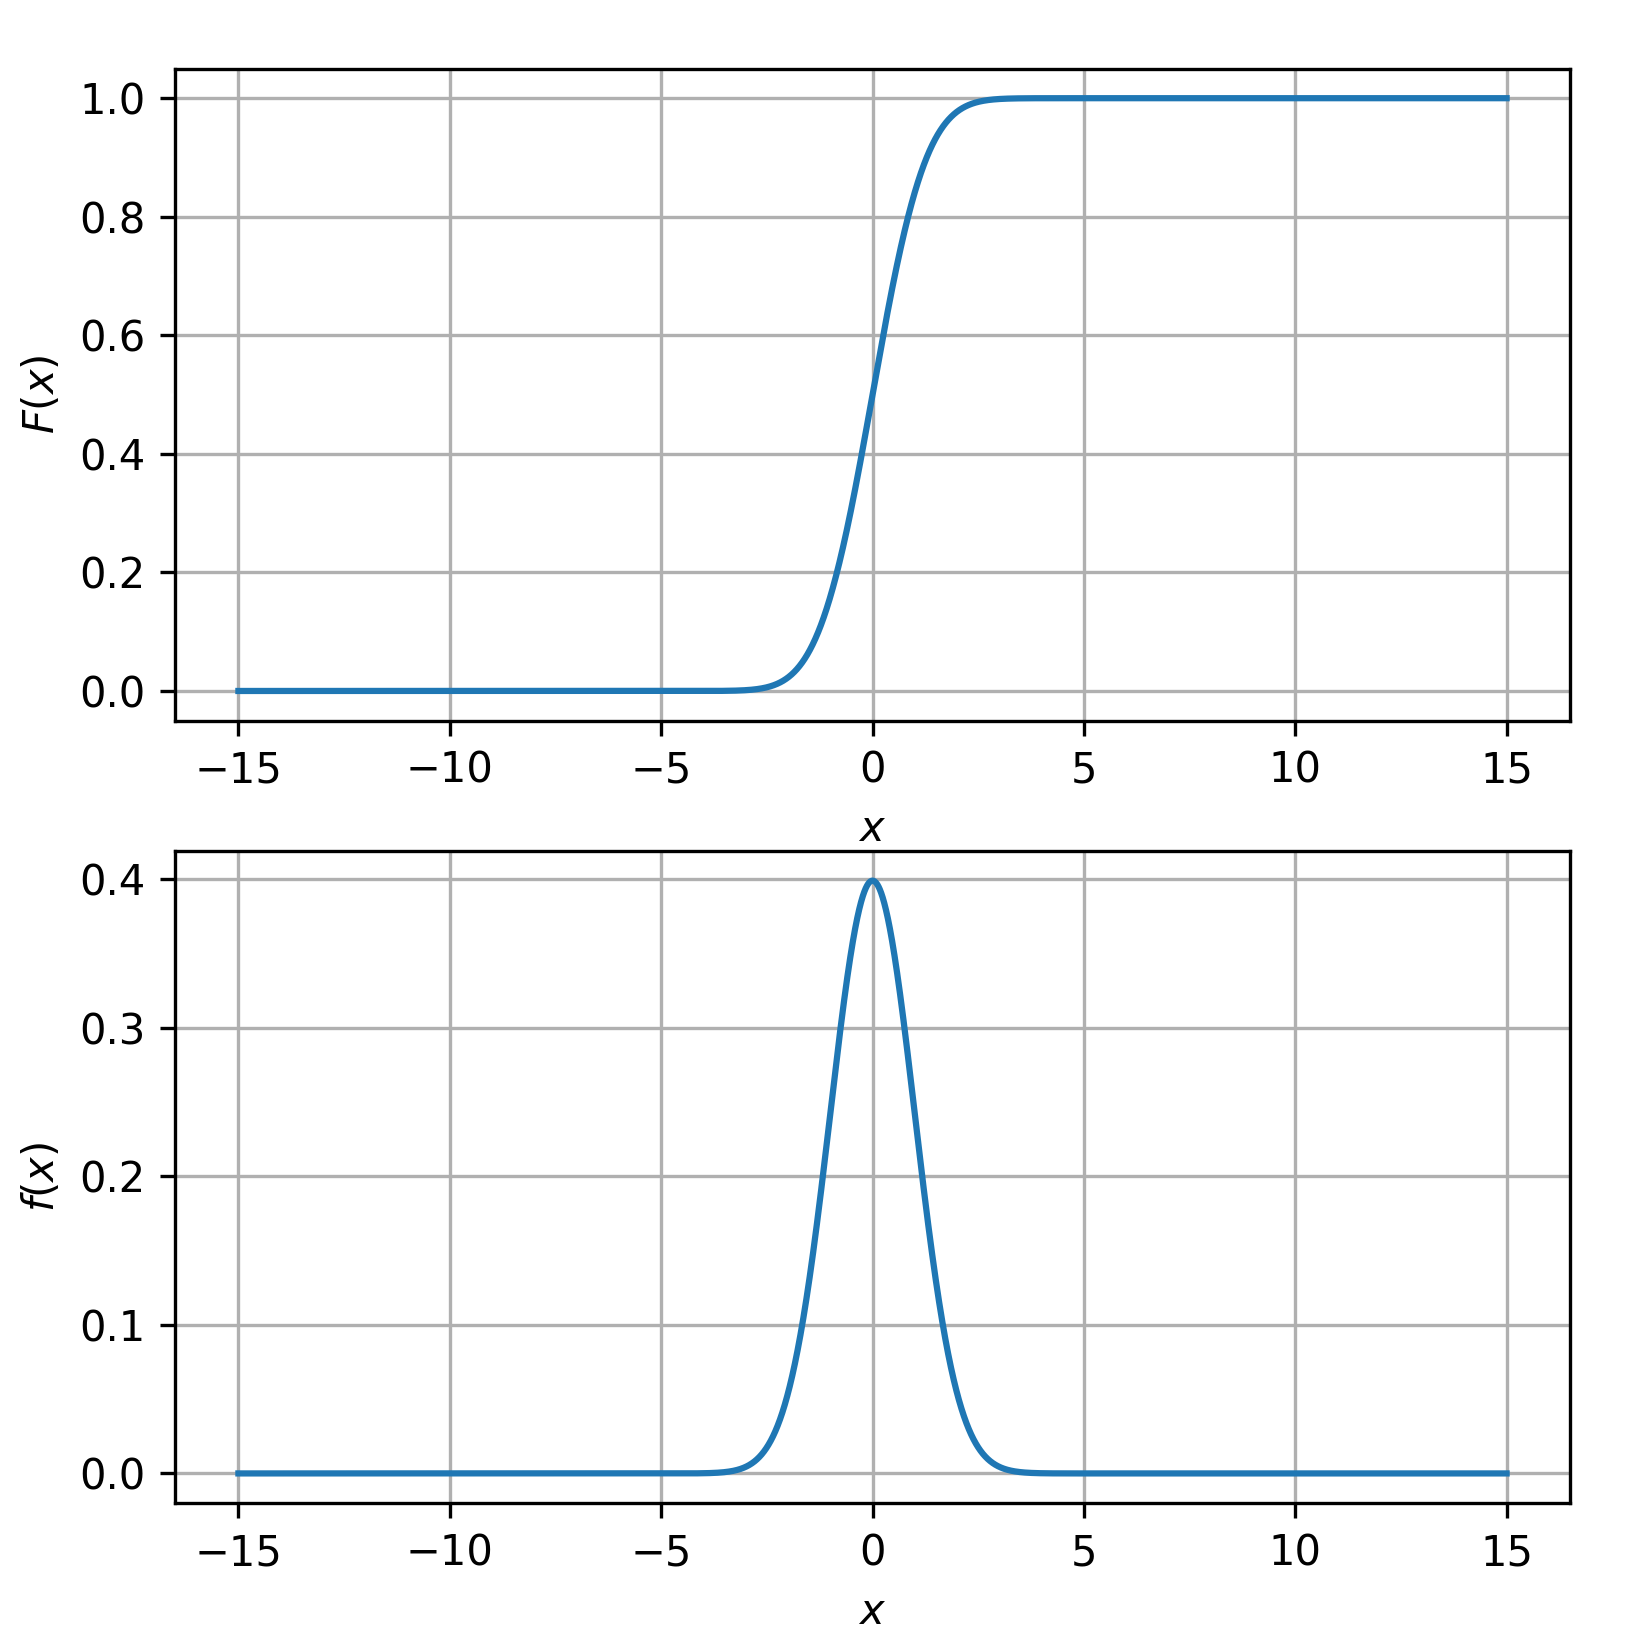
\includegraphics[scale=0.8]{norm1}
	\centering\caption{Нормальное распределение при $\mu$ = 0, $\sigma$ = 1}
\end{figure}
\clearpage
\newpage
\begin{figure}[t!]
	\centering 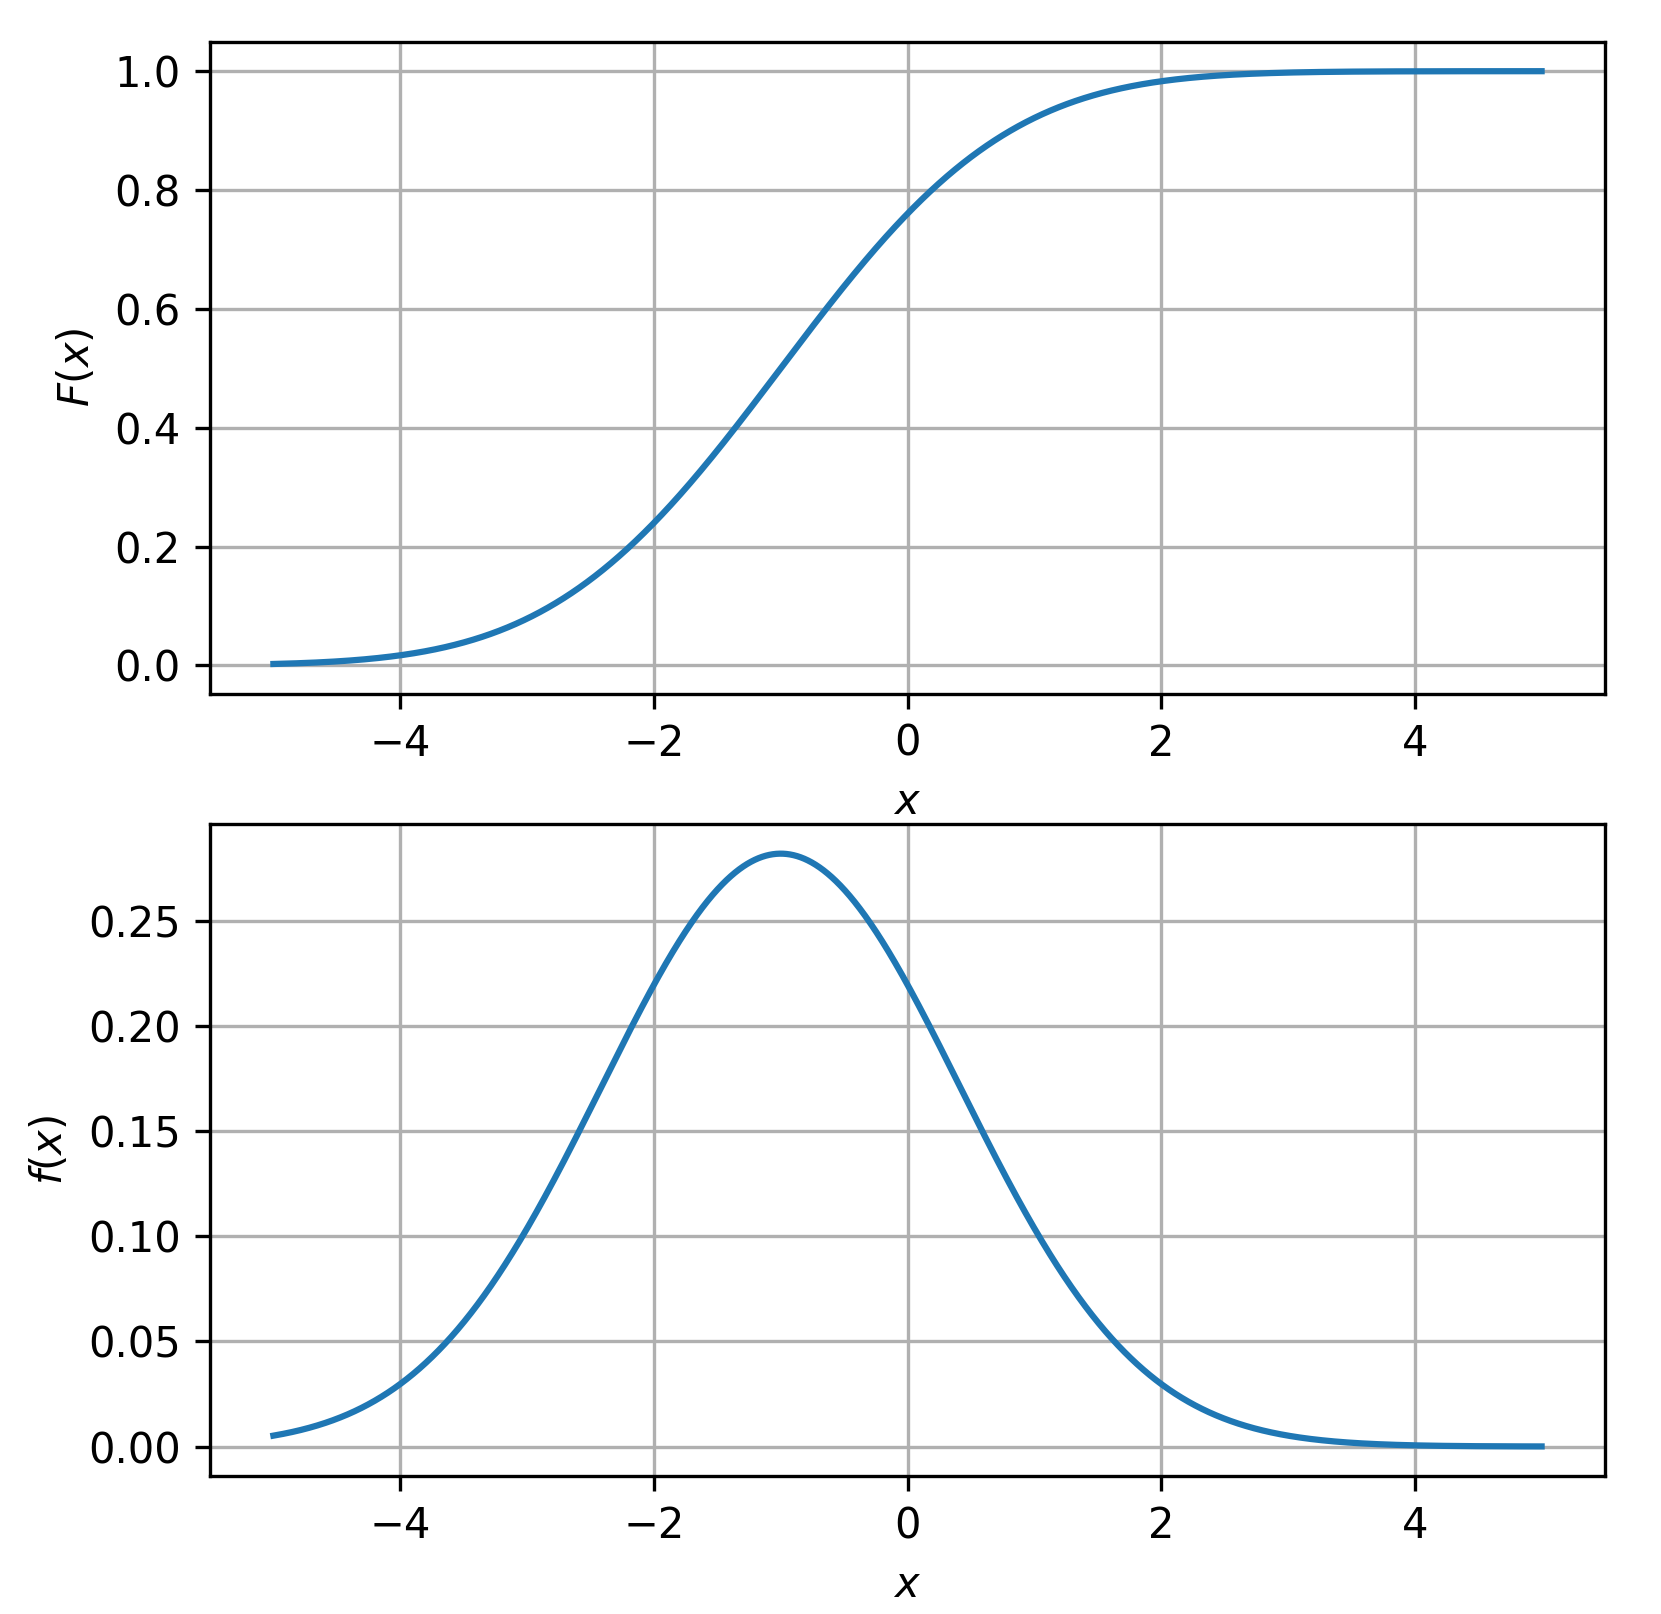
\includegraphics[scale=0.8]{norm2}
	\centering\caption{Нормальное распределение при $\mu$ = -1, $\sigma$ = 2}
\end{figure}
\section{Листинг кода}
\definecolor{codegreen}{rgb}{0,0.6,0}
\definecolor{codegray}{rgb}{0.5,0.5,0.5}
\definecolor{codepurple}{rgb}{0.58,0,0.82}
\definecolor{backcolour}{rgb}{0.95,0.95,0.92}

\lstdefinestyle{mystyle}{
	backgroundcolor=\color{backcolour},   
	commentstyle=\color{codegreen},
	keywordstyle=\color{magenta},
	numberstyle=\tiny\color{codegray},
	stringstyle=\color{codepurple},
	basicstyle=\ttfamily\footnotesize,
	breakatwhitespace=false,         
	breaklines=false,                 
	captionpos=b,                    
	keepspaces=true,                 
	numbers=left,                    
	numbersep=5pt,                  
	showspaces=false,                
	showstringspaces=false,
	showtabs=false,                  
	tabsize=4
}

\lstset{style=mystyle}

\begin{lstlisting}[language=Python, caption = программная реализация равномерного распределения и нормального распределения]
def main():
	a = float(input("Enter start point a: "))
	b = float(input("Enter end point b: "))
	mu = float(input("Enter mu for normal distribution: "))
	sigma = float(input("Enter sigma for normal distribution: "))

	delta = b - a

	x_uniform = np.arange(a - delta / 2, b + delta / 2, 0.001)
	x_normal = np.arange(a, b, 0.001)


	y_uniform_cdf = [uniform_distribution_cdf(a, b, value) 
									for value in x_uniform]
	y_uniform_pdf = [uniform_distribution_pdf(a, b, value) 
									for value in x_uniform]

	y_normal_cdf = normal_distribution_cdf(x_normal, mu, sigma)
	y_normal_pdf = normal_distribution_pdf(x_normal, mu, sigma)

	draw_plots(x_uniform, y_uniform_cdf, y_uniform_pdf)
	draw_plots(x_normal, y_normal_cdf, y_normal_pdf)


def draw_plots(x, y_cdf, y_pdf):
	fig, axs = plt.subplots(2, figsize=(6,7))

	axs[0].plot(x, y_cdf)
	axs[1].plot(x, y_pdf)

	axs[0].set_xlabel('$x$')
	axs[0].set_ylabel('$F(x)$')

	axs[1].set_xlabel('$x$')
	axs[1].set_ylabel('$f(x)$')

	axs[0].grid(True)
	axs[1].grid(True)

	plt.show()


def uniform_distribution_cdf(a, b, x):
	return (x - a) / (b - a) if (a <= x < b) else 0 if x < a else 1

def uniform_distribution_pdf(a, b, x):
	return 1 / (b - a) if (a <= x <= b) else 0

def normal_distribution_cdf(x, mu, sigma):
	return norm.cdf(x, mu, sqrt(sigma))

def normal_distribution_pdf(x, mu, sigma):
	return norm.pdf(x, mu, sqrt(sigma))
\end{lstlisting}
\end{document}